\documentclass[11pt]{article}
\usepackage[T1]{fontenc}
\usepackage{lmodern,microtype}
\usepackage[a4paper,margin=25mm]{geometry}
\usepackage{amsmath,amssymb,amsthm,mathtools,booktabs,graphicx,array,xcolor,xurl}
\usepackage[colorlinks=true,linkcolor=blue!45!black,citecolor=blue!45!black,urlcolor=blue!45!black]{hyperref}
\hypersetup{pdfauthor={Wenyu Huang},pdftitle={Retained Evidence for Changing Predictions}}
\newtheorem{theorem}{Theorem}[section]
\newtheorem{corollary}[theorem]{Corollary}
\newtheorem{proposition}[theorem]{Proposition}
\newtheorem{lemma}[theorem]{Lemma}
\newcommand{\E}{\mathbb E}
\newcommand{\PP}{\mathbb P}
\newcommand{\ip}[2]{\langle #1,#2\rangle_\mu}
\newcommand{\norm}[1]{\lVert #1\rVert}
\DeclareMathOperator{\KL}{KL}
\DeclareMathOperator{\kl}{kl}
\DeclareMathOperator{\Var}{Var}
\DeclareMathOperator{\spanop}{span}
\graphicspath{{figures/}}
\title{Retained Evidence for Changing Predictions\\[4pt]
\large Exact Moment Ambiguity and Fresh-Audit Learning Diagnostics}
\author{Wenyu Huang\\University of California San Diego}
\date{}

\date{Research report, September 2026}
\begin{document}
\maketitle
\begin{abstract}
We investigate two distinct ways to use historical labels during structural
learning: fitting future candidates and certifying their current risks.
For a known finite input law, we derive the exact worst-case ambiguity of a
Brier-risk change given approximate label moments. With exact moments,
prediction movement outside the retained span determines matching upper and
lower fresh-testing orders for symmetric prediction pairs in a stated
small-margin regime. The mathematics
specializes optimal recovery, control variates and sequential testing; it is
not an established new general inference principle. Finite-state experiments
show both the value of oracle retained evidence and the loss caused by its
finite estimation error. A stress test exposes invalid adaptive reuse.
Separately, 336 trained neural trajectories compare permanent audit withholding
with post-decision release, informative and random growth, and same-arrival
fixed-capacity online controls. Release lowers mean final risk for both
proposal mechanisms. Residual proposals show no resolved advantage over
random proposals, while larger fixed learners obtain lower risks on two
nonlinear tasks. These results diagnose a preventable data-use restriction
without proving that structural adaptation is generally superior. Complete
proofs, frozen protocols, raw outcomes and explicit resource limits accompany
the report.
\end{abstract}

\section*{Research status and relation to the preprint candidates}
This September 2026 report contains the analysis and experiments from that
research stage. Repository preparation did not rerun the experiments.
The existing-results preprint candidate, \emph{Evidence Interfaces in Repeated
Neural Growth}, is prepared separately. The present report is material for
scientific study within that line, with its stated assumptions and limits.
The strongest new mathematical result in the coordinated investigation is
a separate matching source-mass order for four-state irreversible finite
representations; it belongs to the finite-representation manuscript.

The motivating distinction is practical. Releasing an old audit into future
fitting does not give a new candidate independent historical certification
data. Conversely, retained information need not become useless merely because
a predictor changes. We quantify the latter point within a fixed moment
interface and test the former in actual trained networks.

\section{Model, information access, and prior work}
Let $X$ have a known law $\mu$ on $\{1,\ldots,m\}$, with $\mu_i>0$. Define
\[
 \ip ab=\sum_i\mu_i a_i b_i,\qquad
 \norm a_p=\Big(\sum_i\mu_i|a_i|^p\Big)^{1/p}.
\]
Labels $Y\in\{0,1\}$ have unrestricted conditional signed mean
$g_i=\E[2Y-1\mid X=i]\in[-1,1]$. A dictionary $B\in\mathbb R^{m\times d}$ is fixed in advance, with columns $b_j$ and span $V$. The exact population-moment interface reveals
\[
 m_j(g)=\ip{b_j}g,\qquad j=1,\ldots,d.
\]
This specifies information access, not physical storage. A real scalar can encode a finite label vector, and even a fixed empirical linear sketch with rationally independent weights can encode integer count vectors. No memory lower bound follows from the dictionary rank. Moreover, the distribution of an empirical summary can contain information absent from its population expectation; our exact-moment lower bound does not automatically apply to that distribution.

For predictions $p,q\in[0,1]^m$, write $h=q-p$ and $c=\ip h{1-p-q}$. Expanding squares yields
\begin{equation}
 \Delta_g(p,q):=\E[(Y-p(X))^2-(Y-q(X))^2]=c+\ip hg.
 \label{eq:gain}
\end{equation}
Only the change $h$ multiplies the unknown label means. The known input law makes $c$ and the approximation geometry computable. Unknown $\mu$ requires additional uncertainty control.

Control-variate confidence intervals already estimate the residual after subtracting a variable with known mean \cite{zhao2020}; projection-based residual concentration and coefficient-error analysis are established \cite[Eq.~(6), Theorem~3.1, Appendix~B]{leluc2021}. Uniform confidence regions accommodate adaptive use \cite[Theorem~3, Corollary~1]{abbasi2011}. In structural learning, Amoukou et al.\ already certify current prediction-risk differences by minimizing over a stationary probability region \cite[Lemma~A.13]{amoukou2026}. Our analysis specializes these tools and a standard testing lower bound \cite[Lemma~1]{kaufmann2016} to retained label moments. Convex duality is used in its standard form \cite{boyd2004}.

\section{Sharp reconstruction from approximate moments}
Suppose $z\in\mathbb R^d$ is known to satisfy $|z_j-m_j(g)|\le e_j$, where $e_j\ge0$. For fixed $h$, let
\[
 \mathcal R(h,B,e)=\inf_T\ \sup_{\substack{g\in[-1,1]^m\\|z-m(g)|\le e}}
       |T(z)-\ip hg|,
\]
where the supremum includes all admissible $(g,z)$ and the infimum allows arbitrary functions $T$, including nonlinear ones.

\begin{theorem}[Exact ambiguity of retained moments]\label{thm:ambiguity}
One has
\begin{align}
 \mathcal R(h,B,e)
 &=\max_{\substack{\norm u_\infty\le1\\|B^\top\operatorname{diag}(\mu)u|\le e}}\ip hu\label{eq:primal}\\
 &=\min_{a\in\mathbb R^d}\left\{\norm{h-Ba}_1+\sum_j e_j|a_j|\right\}.
 \label{eq:dual}
\end{align}
In particular, $\mathcal R(h,B,0)=\operatorname{dist}_{L_1(\mu)}(h,V)$, which is zero if and only if $h\in V$.
\end{theorem}
\begin{proof}
For any $a$, the estimator $T(z)=a^\top z$ obeys
\[
 |T(z)-\ip hg|
 \le\norm{h-Ba}_1+\sum_j e_j|a_j|.
\]
For a lower bound take $z=0$. Every feasible $u$ in \eqref{eq:primal}, as well as $-u$, is consistent with $z=0$. Their target values are opposite, so one of the two errors of any $T(0)$ is at least $|\ip hu|$. The feasible set is nonempty, symmetric and compact.

It remains to equate \eqref{eq:primal} and \eqref{eq:dual}. Assign nonnegative multipliers $s,t$ to the upper and lower moment constraints in the maximization. Maximizing its Lagrangian over $[-1,1]^m$ yields
\[
 \norm{h-B(s-t)}_1+e^\top(s+t).
\]
For fixed $a=s-t$, the smallest second term is $\sum_j e_j|a_j|$, attained by the positive and negative parts of $a$. Finite linear-program strong duality applies: the primal is feasible with finite optimum and the dual is feasible, for example at $a=0$. This proves equality and attainment. Finally, finite-dimensional $V$ is closed, so its $L_1$ distance is zero exactly on $V$. Adding the known $c$ in \eqref{eq:gain} does not change any error.
\end{proof}

\begin{corollary}[No-data decision obstruction]
Let $\norm h_\infty\le1$ and $h\notin V$. Symmetric predictions
$p=(1-h)/2$, $q=(1+h)/2$ admit two binary-label laws with identical exact retained moments and strictly opposite gains. No randomized rule based solely on these moments can have type-I error at most $\alpha$ and power at least $1-\beta$ on both laws when $\alpha+\beta<1$.
\end{corollary}
\begin{proof}
With $e=0$, choose a maximizer $u$ of \eqref{eq:primal}. Set $g=\pm u$. Both give zero moments, while $c=0$ and the gains are
$\pm\operatorname{dist}_{L_1(\mu)}(h,V)$. The acceptance probability is the same under both indistinguishable observations; the two requirements would give $1-\beta\le\alpha$.
\end{proof}

\section{The additional cost of fresh evidence}
Let $v$ be the $L_2(\mu)$ projection of fixed $h$ onto $V$, and put
\[
 r=h-v,\qquad S=\norm r_2^2,\qquad M=\norm r_\infty.
\]
Exact moments determine $A=c+\ip vg$. On $n$ fresh iid full pairs, define
\[
 \widehat\Delta=A+\frac1n\sum_{i=1}^n r(X_i)(2Y_i-1).
\]

\begin{theorem}[Residual upper bound]\label{thm:upper}
For $u>0$ and $n\ge1$, let
\[
 F_n(u)=\sqrt{\frac{2Su}{n}}+\frac{4Mu}{3n}.
\]
Then $\PP(|\widehat\Delta-\Delta|>F_n(u))\le2e^{-u}$, with failure probability $e^{-u}$ for either one-sided endpoint. Accepting when $\widehat\Delta>F_n(u)$ has type-I error at most $e^{-u}$ for $\Delta\le0$. For $\Delta\ge\gamma>0$, it has power at least $1-e^{-u}$ whenever
\begin{equation}
 n>\max\left\{\frac{32Su}{\gamma^2},\frac{16Mu}{3\gamma}\right\}.
 \label{eq:upper-n}
\end{equation}
If $S=0$, the gain is exactly known and no fresh data are required.
\end{theorem}
\begin{proof}
If $S=0$, positivity of every $\mu_i$ implies $r=0$, so the gain is exactly known. Assume $S>0$, hence $M>0$. Write $W=r(X)(2Y-1)$ and $Z=W-\E W$. Then
$\E W^2=S$, $\Var(W)\le S$, and $|Z|\le2M$. For $k\ge2$,
$\E|Z|^k\le(2M)^{k-2}\E Z^2$. The exponential series, $k!\ge2\cdot3^{k-2}$, and $\log(1+x)\le x$ give
\[
 \log\E e^{\lambda Z}
 \le\frac{\lambda^2S}{2(1-2M|\lambda|/3)},
 \qquad |\lambda|<3/(2M).
\]
For $t>0$ choose $\lambda=t/(S+2Mt/3)$ in the exponential Markov bound for the sum of $n$ independent copies, obtaining
\[
 \PP\left(\frac1n\sum_i Z_i\ge t\right)
 \le\exp\left\{-\frac{nt^2}{2(S+2Mt/3)}\right\}.
\]
Substitution of $F_n(u)$ makes the exponent at least $u$. Repeat for $-Z$. The strict sample condition \eqref{eq:upper-n} makes both terms of $F_n$ less than $\gamma/4$. On the lower-tail coverage event, $\widehat\Delta\ge\Delta-F_n>F_n$. If $S=0$, positivity of every $\mu_i$ implies $r=0$, proving the final statement.
\end{proof}

\begin{theorem}[Matching residual lower bound]\label{thm:lower}
Suppose $\norm h_\infty\le1$, $S>0$, and
\[
 0<\gamma\le \frac{S}{2M},\qquad
 \alpha,\beta\in(0,1),\quad\alpha+\beta<1.
\]
Use symmetric predictions $p=(1-h)/2$, $q=(1+h)/2$. A test receives exact $V$-moments, then observes a fresh iid stream of full $(X,Y)$ pairs, and may randomize and stop sequentially. Suppose it stops almost surely under the laws constructed below, has acceptance probability at most $\alpha$ under every law with $\Delta\le0$, and at least $1-\beta$ under every law with $\Delta\ge\gamma$. There is a law with gain exactly $\gamma$ under which
\begin{equation}
 \E N\ge \kl(1-\beta,\alpha)\frac{S}{\gamma^2}.
 \label{eq:lower-n}
\end{equation}
\end{theorem}
\begin{proof}
Under $P_0$ set $g=0$; under $P_1$ set $g=\gamma r/S$. The size condition gives $|g_i|\le1/2$, so both laws have conditional Bernoulli means in $[1/4,3/4]$. Orthogonality gives $\ip{b_j}r=0$, so the exact initial moment vector is zero under both laws. Also $c=0$ and
\[
 \Delta_0=0,\qquad
 \Delta_1=\frac\gamma S\ip hr=\gamma,
\]
using $\ip hr=\norm r_2^2=S$.

The elementary inequality
$\kl(a,b)\le(a-b)^2/[b(1-b)]$ follows from applying $\log x\le x-1$ to the two logarithms. Therefore
\begin{align*}
 \KL(P_1,P_0)
 &=\sum_i\mu_i\kl\left(\frac{1+\gamma r_i/S}{2},\frac12\right)\\
 &\le\sum_i\mu_i\left(\frac{\gamma r_i}{S}\right)^2
 =\frac{\gamma^2}{S}.
\end{align*}
If $\E_1N=\infty$, the claim is immediate. Otherwise, the stopped log-likelihood ratio equals
\[
 \sum_{i\ge1}\mathbf1_{\{N\ge i\}}
       \log\frac{dP_1}{dP_0}(X_i,Y_i).
\]
The likelihood increments are bounded, the expectation of $N$ is finite, and $\{N\ge i\}$ is measurable before draw $i$. Absolute integrability and conditional expectation show that the stopped-transcript divergence equals $\E_1N\KL(P_1,P_0)$. The common stopping and randomization rule contributes no additional likelihood factor. By data processing onto the acceptance event and binary-KL monotonicity,
\[
 \E_1N\KL(P_1,P_0)
 \ge\kl(P_1(\mathrm{accept}),P_0(\mathrm{accept}))
 \ge\kl(1-\beta,\alpha).
\]
Combining the inequalities proves \eqref{eq:lower-n}.
\end{proof}

For $\alpha=\beta=\delta\le1/4$, the binary divergence is
$(1-2\delta)\log((1-\delta)/\delta)$, of order $\log(1/\delta)$. The small-margin condition gives $M/\gamma\le S/(2\gamma^2)$, absorbing the range term in the upper bound. Thus, for symmetric prediction pairs in this small-margin regime, the minimax additional testing cost for this fixed exact-moment interface has order
\[
 S\gamma^{-2}\log(1/\delta).
\]
The lower construction is a problem-specific specialization of the standard sequential change-of-measure method, not a new testing principle. It does not allow arbitrary additional informative training histories: their divergence could pay for part of the decision.

\section{Finite historical evidence and adaptive pairs}
Fix the dictionary before an old iid sample $H$ of size $N_0$, and assume $|b_j|\le B_j$. Retain
\[
 z_j=\frac1{N_0}\sum_{i=1}^{N_0}b_j(X_i)(2Y_i-1),\qquad
 e_j=B_j\sqrt{\frac{2\log(2d/\delta_0)}{N_0}}.
\]
Hoeffding's inequality and a union bound give probability at least $1-\delta_0$ for the event $\mathcal E_0$ on which every $|z_j-m_j(g)|\le e_j$. All future fitting and pair selection may depend on $H$.

At event $t$, condition on pre-audit history and select $p_t,q_t,a_t,n_t$. Put $v_t=Ba_t$, $r_t=q_t-p_t-v_t$, $c_t=\ip{q_t-p_t}{1-p_t-q_t}$, and
\[
 H_t=\sum_j e_j|a_{tj}|,\quad
 F_t=\sqrt{\frac{2\norm{r_t}_2^2\log(1/\delta_t)}{n_t}}
       +\frac{4\norm{r_t}_\infty\log(1/\delta_t)}{3n_t}.
\]
Using a new independent audit, define
\[
 L_t=c_t+a_t^\top z+\frac1{n_t}\sum_{i=1}^{n_t}
       r_t(X_{ti})(2Y_{ti}-1)-H_t-F_t.
\]
\begin{proposition}[Adaptive transfer with historical uncertainty]
For a finite or countable sequence of such events,
\[
 \PP(\exists t:L_t>\Delta_t)\le\delta_0+\sum_t\delta_t.
\]
\end{proposition}
\begin{proof}
On $\mathcal E_0$, the deterministic inequality
$|a^\top(z-m(g))|\le\sum_j e_j|a_j|$ holds for every $a$, hence for adaptive $a_t$. Conditional on each pre-audit history, the residual is fixed and Theorem~\ref{thm:upper} bounds the fresh one-sided failure by $\delta_t$. Integrate and take a union bound together with $\mathcal E_0^c$. Countable unions follow by increasing finite unions.
\end{proof}

The proposition is a standard simultaneous-region argument, with a direct structural-learning precedent \cite[Lemma~A.13]{amoukou2026}. It transfers estimates together with their uncertainty, not old betting products. New dictionary columns fitted on old labels require a uniform class argument or fresh data. Completed audits may later enter fitting while future audit blocks remain independent. Refreshing the inference region across update times needs simultaneous bounds for those updates. When historical errors are nonzero, the $L_2$ projection need not minimize $H_t+F_t$; shrinking $a_t$, including to zero, can be preferable. If $r_t=0$, residual-only future auditing cannot shrink $H_t$.



\section{Releasing completed audits into later fitting}
\begin{proposition}[Standard conditional-validity corollary]
Let $\mathcal H_{t-1}$ contain every earlier fitting sample, completed audit,
decision and optimizer state. Before revealing audit $A_t$, construct the
incumbent and all candidate predictors measurably from $\mathcal H_{t-1}$ and
independent proposal randomness. Suppose $A_t$ is iid from the task law,
independent of the complete pre-audit sigma field, including proposal
randomness, and the conditional probability of a falsely
accepted comparison is at most $\alpha_{tj}$, with predictable total
$\sum_{t,j}\alpha_{tj}\le\delta$. Commit only the chosen frozen candidate,
or hold the incumbent exactly. Then with probability at least $1-\delta$
every accepted inequality holds in population. After committing, $A_t$ may
enter $\mathcal H_t$ and any future fitting pool.
\end{proposition}
\begin{proof}
Condition on the full pre-audit history and proposal randomness. Current
predictors are fixed and the audit remains independent, so the stipulated
conditional error bound applies. Integrate over history and sum the error
bounds. This yields a simultaneous event on which every installed change
satisfies its audited inequality. Label release changes later history, not
the conditional argument for a genuinely fresh later block. A hold changes
neither predictor nor risk. Increasing finite unions cover a countable
sequence. No candidate-discovery or power statement follows.
\end{proof}
This is the same standard fresh-evidence reasoning used by the inherited
controller; the new item is its implemented diagnostic. A silent refit of the
installed predictor would break the claimed checkpoint protection. Optimizer
state may persist, but its resulting fitted parameters must still be audited
before installation. Ordinary ungated online learners and diagnostic training
tails pursue a different objective and have no such guarantee.

\paragraph{Why a previous betting product is not a new-pair certificate.}
Consider a single input and $Y\sim\mathrm{Bernoulli}(3/4)$. The old pair
$p=1/4,q=3/4$ has difference $D=\tfrac12(2Y-1)$ and positive gain.
Its product with bet $1/2$ has positive expected log increment
$\tfrac34\log(5/4)+\tfrac14\log(3/4)>0$ and therefore crosses any fixed
threshold almost surely. Swapping the pair makes the true gain negative.
Using the old product as its initial evidence would accept the harmful new
pair with probability one if no new evidence were required. Even after one
fresh factor, choosing the old threshold larger by $4/3$ preserves that
counterexample. This does not contradict a prequential test whose null bounds
every conditional increment; that is a different hypothesis. The valid
transfers above retain a confidence region with its uncertainty.

\section{Finite-state experiments on retained evidence}
\subsection{Frozen design and supplemental controls}
The R1 protocol fixes a uniform four-state input $(f_1,f_2)\in\{-1,1\}^2$,
$h=0.2(\sqrt{1-z}f_1+\sqrt z f_2)$, and symmetric predictions
$p=(1-h)/2,q=(1+h)/2$. The retained span is $V=\mathrm{span}(f_1)$.
The squared total movement is $0.04$ and residual movement $0.04z$ for
$z\in\{1,1/4,1/16,1/64\}$. The null has $\eta=1/2$; alternatives have
$\eta=1/2+0.003f_2/(0.4\sqrt z)$, giving the same gain $0.003$.
All probabilities lie in $[1/4,3/4]$.

For each condition, 1,000 independent replicates generate nested iid count
samples at six fixed fresh sizes from 128 to 131,072. Methods use a direct
paired Bernstein bound, a residual bound with an exact oracle moment, or a
residual bound with 32,768 independent historical labels and a Hoeffding
moment interval. The finite-history method divides error $0.05$ equally
between historical and fresh uncertainty. The oracle's exact moment is
privileged information, not a free finite dataset. Displayed rejection rates
are pointwise at fixed sizes; the plotted grid is not a valid repeated-look
test without additional allocation.

An explicitly post-hoc supplement adds two necessary controls from the
unchanged archived counts. Because the R1 pair is precommitted, a direct
comparison can use all old and fresh labels. A second control selects a
shrunken retained coefficient by minimizing the analytic historical-plus-fresh
radius using only geometry and sample sizes, before inspecting observed
values. These controls preserve the frozen results and do not create a new
confirmatory comparison.

\begin{figure}[tb]
\centering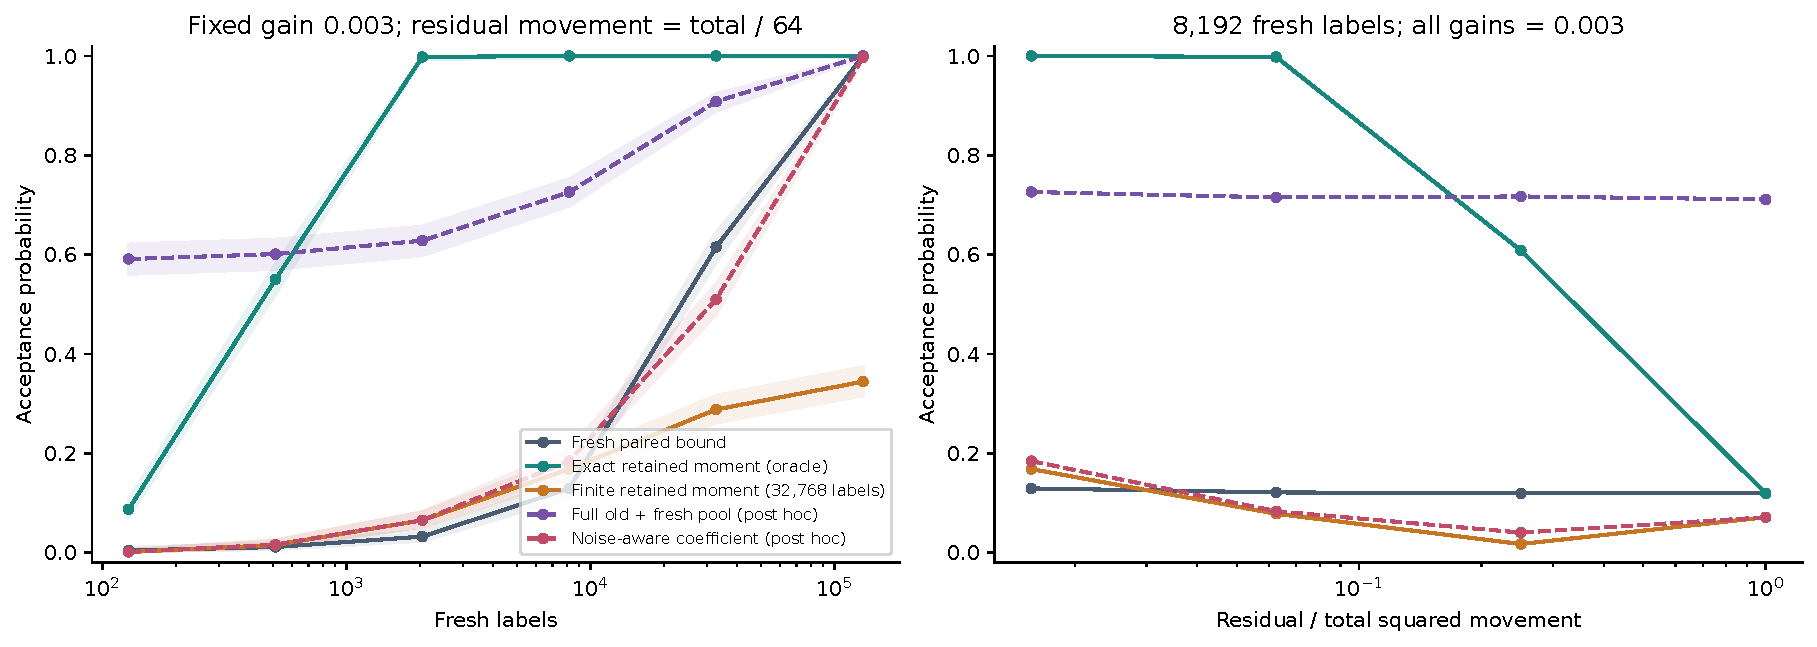
\includegraphics[width=\linewidth]{retention_geometry.pdf}
\caption{R1: genuine finite-state sampling, not neural training. Bands are
pointwise 95\% Wilson intervals over 1,000 independent replicates. Dashed
methods were added after viewing the frozen results. Full-pool and finite
history methods both use 32,768 additional historical labels; the oracle
moment is a separate ideal-information resource.}
\end{figure}

At $z=1/64$ and 8,192 fresh labels, direct testing accepts in 129 of 1,000
alternative replicates, exact-moment residual testing in 1,000, and the
finite-history method in 168. The oracle result verifies the predicted
mechanism, while the finite-history result prevents claiming the same
efficiency for a realizable procedure. The full-pool comparator also makes
clear that compressing history can lose useful evidence. A fixed imperfect
retained projection leaves historical uncertainty even when residual evidence
becomes abundant; shrinking toward zero avoids that particular floor.

\subsection{Adaptive reuse stress test}
R2 has $m\in\{4,16,64\}$ equiprobable inputs and the null law $\eta=1/2$.
After 4,096 historical observations, it chooses
$h_j=0.4\,\mathrm{sign}(\widehat{\E}[1_{X=j}(Y-1/2)])$ and symmetric
predictions. Every selected pair has true gain zero. Across 1,000 new
replicates, we compare naive fixed-pair Bernstein reuse, a simultaneous
coordinate moment region, and 4,096 genuinely fresh labels conditional on
the selected pair. The moment region is deliberately elementary and can be
conservative; this null stress test makes no power claim for it.

Naive reuse falsely accepts 69, 880 and 1,000 times as $m$ increases; fresh
audits accept 3, 6 and 2 times, and the simultaneous region accepts zero.
Zero observed failures do not prove zero error probability. The experiment
is a designed selection-bias diagnostic, not a claim that typical neural
training exhibits those false-acceptance rates.

\begin{figure}[tb]
\centering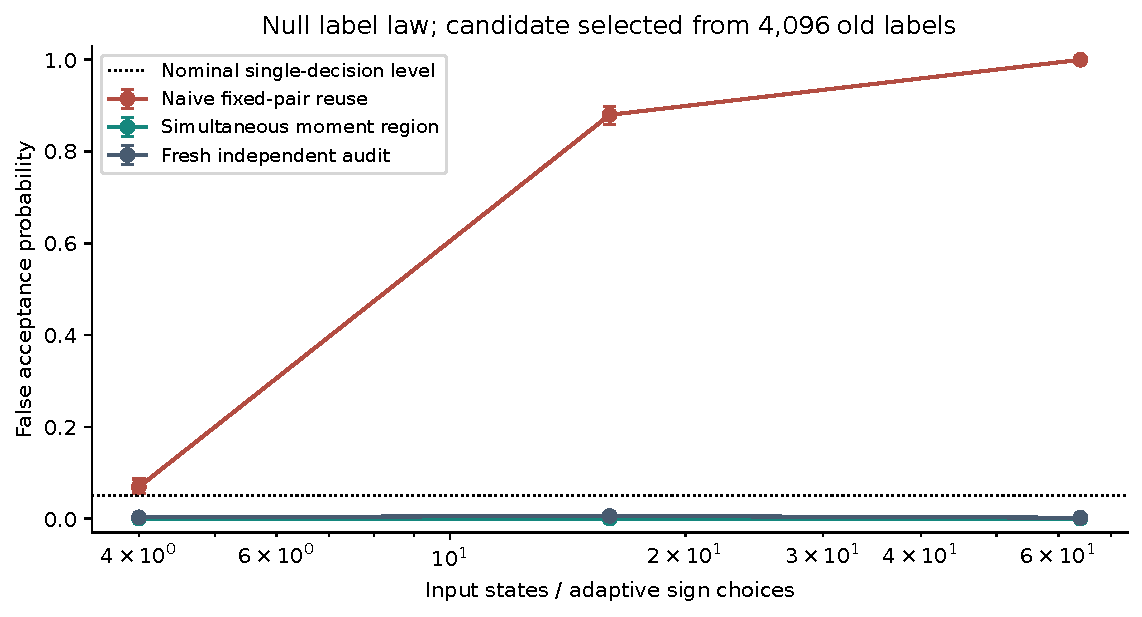
\includegraphics[width=.88\linewidth]{adaptive_reuse.pdf}
\caption{R2: the new candidate is chosen using the old labels. Error bars
are Wilson intervals across independent replicates. Ordinary fixed-pair
coverage cannot be applied retrospectively to that selected comparison.}
\end{figure}

% Self-contained experimental section. Requires amsmath, amssymb, graphicx,
% booktabs, hyperref. Define \experimentroot if this file is included elsewhere.
\providecommand{\experimentroot}{.}
\section{Completed audits as future fitting data}
\label{sec:audit-release-diagnostic}

The following new-seed diagnostic asks whether permanently excluding completed
audits from later fitting creates avoidable limitations in a trained adaptive
learner. It does not claim a new testing theorem, and it does not implement
transfer of historical certification evidence to a changed prediction pair.
The broad motivation is useful structural adaptation under explicit data and
computation costs; success of the residual proposal is not assumed.

\subsection{Implemented evidence mechanism}
Let $H_{t-1}$ contain every earlier fitting/audit observation, decision,
parameter and optimizer state. Current proposal randomness may be included
before the next audit. Suppose all current predictors and comparison margins
are then fixed and the current block $A_t$ is independent and iid. For old
minus new bounded-loss differences $D_i\in[-1,1]$, define
\[
 E_n=\frac15\sum_{\lambda\in\Lambda_\tau}
       \prod_{i=1}^n\{1+\lambda(D_i-\tau)\},\qquad
 \Lambda_\tau=\{.05,.1,.2,.5,(1+\tau)^{-1}\},
\]
with the implemented margins $\tau\in\{0,.0005\}$.
Accept the inequality when $E_n\ge 1/\alpha_{t,j}$. This is an established
bounded-mean betting construction, not a new test; the direct foundation is
Waudby-Smith and Ramdas, Section~4 and Appendix~A.3 of the inspected
arXiv version~7 \cite{waudby2024}.

Each product has nonnegative factors and conditional expectation at most one
under its null. Its fixed average therefore gives the conditional error bound
needed by the preceding proposition. Every changed prediction pair starts a
new product. The current experiment uses fixed blocks, with no uncorrected
multiple inspections within a block.

\subsection{Frozen design and actual execution}
The protocol and runner hashes were frozen at 03:45:05 UTC on
15 September 2026, before seeds 750000--750011 were run. Four tasks and
12 independent seeds per task give 48 paired configurations, seven methods
per configuration, 336 complete trajectories and 8,064 events. All completed
the preset 24-event horizon. The main run took 330.7 seconds with two local
CPU workers. An unchanged-runner recovery of the earlier interaction seed
63000 matched its full two-method history and controls before this study.

Write $\sigma(u)=1/(1+e^{-u})$. All tasks have $X\sim N(0,I_6)$ and
$Y\mid X\sim\operatorname{Bernoulli}(.05+.9\sigma(g(X)))$, where
\begin{align*}
g_{\rm null}(x)&=0,\\
g_{\rm additive}(x)&=2.5\tanh(2x_1+.6)-2\tanh(2x_2-.5)
 +1.7\tanh(2x_3+.3)-1.5\tanh(2x_4),\\
g_{\rm interaction}(x)&=4\tanh(2x_1)\tanh(2x_2)
 +2\tanh(2x_3)\tanh(2x_4),\\
g_{\rm radial}(x)&=3(x_1^2+x_2^2-1.4).
\end{align*}
The radial boundary is an additional task with four nuisance coordinates,
not an instance of a supplied-module theorem. The fitted network is
$p_\theta(x)=\sigma(c+\sum_{j=1}^k a_j\tanh(w_j^\top x+b_j))$ with Brier
loss; all its parameters train. There are 2,048 initial fitting labels and
4,096 fresh audit labels at each event, hence 100,352 unique observed labels
per method. Conditional label noise is integrated on 32,768 independent
evaluator inputs per seed; the risk estimate remains Monte Carlo in $X$.
The evaluator is called only after an entire method's action sequence is
fixed and is absent from the learner's arguments.

Four adaptive arms cross withheld/released audit data with residual/random
proposals. The residual score is
$(\overline{rz})^2/(\overline{z^2}+10^{-3})$, where
$r=y-p$ and $z=p(1-p)\tanh(w^\top x+b)$. Four incoming-vector candidates
receive 40 minibatch ascent updates, and one is selected on at most 4,096
historical fitting points. Random additions use the same initial candidate
distribution and random selection. Both add a unit with outgoing weight
zero, preserving the current predictor before branch fitting. Each event
fits both continuation and growth from the incumbent. Growth is accepted
only after its gains over both incumbent and continuation exceed .0005;
otherwise a certified positive continuation is accepted, or the incumbent
is held exactly.

Three controls receive the same label arrivals and release times: persistent
online learners at fixed widths two and 26, and a fixed width-26 learner
using a fresh gate on continuation. Width 26 equals the adaptive maximum
$2+24$ and is specified before outcomes. The ungated controls make no
checkpoint-monotonicity claim. The adaptive arms allocate $.05/(3\cdot24)$
to each comparison and the one-comparison fixed gate $.05/24$, both spending
the same trajectory error budget. That budget is not a simultaneous
guarantee across experimental methods and seeds.

All arms receive six million parameter--example updates for warmup and
eight million per event, including candidate search and rejected branches,
with small integer remainders recorded. They use persistent Adam
$(.9,.999)$, learning rate .01, denominator constant $10^{-8}$ and minibatches
of at most 256. Proposal ascent uses learning rate .04. Branches clone the
incumbent's optimizer state; only the selected branch commits it. New-unit
moments start at zero and retain the existing step counter. Random proposals
allocate saved search work to branch fitting. Fixed learners devote the
entire event budget to continuation. The 198-million-update horizon and
32-million-update ungated tail match an operation proxy, not FLOPs, optimizer
steps, memory or wall time. These shared persistent-minibatch conventions
differ from the earlier full-batch/reset runner; the new factorial comparison
isolates release within the new protocol.

\subsection{Observed release effects and negative controls}
Table~\ref{tab:release-effects} reports primary paired effects. Confidence
intervals are descriptive 95\% Student-$t$ intervals across the 12 independent
seeds; there is no multiplicity adjustment. Event time points and proposals
are not treated as independent replications.

\begin{table}[tb]
\centering\scriptsize
\begin{tabular}{lrrr}
\toprule
Task & Release: residual & Release: random & Residual minus random\\
\midrule
Null & $-1.994\;[-2.813,-1.176]$ & $-2.016\;[-2.846,-1.186]$ & $0.022\;[-0.054,0.097]$\\
Additive & $-4.576\;[-6.648,-2.505]$ & $-3.943\;[-5.666,-2.221]$ & $0.063\;[-0.237,0.363]$\\
Interaction & $-3.721\;[-4.557,-2.885]$ & $-4.657\;[-6.277,-3.038]$ & $-0.110\;[-0.744,0.524]$\\
Radial & $-1.142\;[-2.131,-0.152]$ & $-1.199\;[-2.081,-0.318]$ & $0.554\;[-0.171,1.280]$\\
\bottomrule
\end{tabular}
\caption{Final Brier-risk differences, in units of $10^{-3}$, with descriptive
95\% paired intervals. ``Release'' means released minus withheld. The last
column compares proposals under release. Negative values favor the first
method. All four release-by-proposal interaction intervals also contain zero.}
\label{tab:release-effects}
\end{table}

Both proposal mechanisms benefit from release in the four measured means.
Their released comparison does not resolve a residual-proposal advantage;
intervals containing zero do not establish equivalence. Mean released
residual final risks are .250716, .131908, .144304 and .121427 on null,
additive, interaction and radial, with respective widths two, four, six and
three. Permanently withheld residual risks are .252710, .136484, .148025 and
.122568. Improvement therefore need not be accompanied by additional
growth: mean interaction width remains six under both release policies.

The fixed width-26 online learner has final mean risks .250857, .131491,
.137553 and .117145. Released residual minus this control is
$+.006752\;[.006203,.007300]$ on interaction and
$+.004282\;[.003656,.004907]$ on radial. Even the gated fixed architecture
outperforms released residual in those comparisons:
$+.003801\;[.003225,.004378]$ and
$+.002762\;[.002014,.003509]$, respectively. Thus removal of the gate is not
the sole explanation for these fixed-capacity results. Fixed width two is
strong on null (mean .250107) but underfits interaction (.209650) and radial
(.192170). The larger control is needed for credible attribution.

After the preset ungated tail, released residual risks become .250161,
.131254, .142542 and .118292. The release-minus-withheld effects remain
negative, but the interaction/radial gaps to fixed26 online remain
$+.004743\;[.004021,.005464]$ and
$+.001445\;[.001061,.001829]$. On additive, this post-training comparison
instead favors the smaller released residual network by
$-.000329\;[-.000491,-.000167]$. These tails are diagnostics, not protected
deployment updates. All adverse and favorable task outcomes are retained.

\begin{figure}[tb]
\centering\includegraphics[width=\linewidth]{\experimentroot/figures/risk_trajectories.pdf}
\caption{Actual 24-event histories; curves are seed means and bands are
$\pm1$ standard error. Released labels improve the adaptive arms, while
fixed-capacity controls expose both underfitting at width two and stronger
risk performance at width 26. All arms share data arrivals and optimization
proxy budgets.}
\label{fig:release-trajectories}
\end{figure}

\subsection{Resource ledger and verification}
Only 96,256 labels have been released before fitting the final online
candidates; the last audit is released after that decision. Withheld arms
fit on exactly 2,048 distinct labels. Released adaptive arms fit on roughly
96,061--96,256, while fixed26 fits about 90,625--90,644 within its matched
parameter--example budget. Repeated fit accesses still differ: released
residual averages 9.84m, 6.36m, 4.71m and 7.31m across tasks, versus .947m
for fixed26 and 11.647m for fixed2. Pool availability is not silently
equated with actual fitting access.

Residual candidate optimization costs 6.881m parameter--example updates over
the horizon. Rejected branch fits alone average 168.727m--182.226m for
released residual. Audit prediction work adds 5.800m--14.090m
parameter--example evaluations, versus 41.091m for fixed26 gated. Adaptive
gates perform 1,474,560 betting-factor evaluations per trajectory; fixed26
gated performs 491,520. Prediction and selection work is logged separately.
The adaptive networks have substantially lower inference capacity than
fixed26, so lower fixed-model risk is a resource tradeoff rather than a
universal dominance statement.

Independent reconstruction from the raw data and saved branch parameters
checks all 8,064 events, 14,976 betting comparisons and evaluator risks;
maximum log-e discrepancy is $9.95\times10^{-13}$. All 48 run hashes,
336 access ledgers and four frozen files pass integrity checks. A separate
full seven-arm interaction replay matches all 168 events at relative
tolerance $10^{-10}$ and absolute tolerance $10^{-12}$, excluding elapsed
times. Checks also verify gradients, function-preserving additions, frozen
candidate hashes, immutable commitments, post-decision release and
current/future-label perturbations. No gated checkpoint increases the
evaluator's estimated risk in this sample; that observation is not the
conditional proof.

\begin{figure}[tb]
\centering\includegraphics[width=\linewidth]{\experimentroot/figures/paired_diagnostics.pdf}
\caption{Prespecified paired final-risk contrasts. Bars are descriptive
95\% intervals across independent seeds, without multiplicity correction.
The scale is $10^{-3}$ Brier-risk units.}
\label{fig:release-paired}
\end{figure}

\begin{figure}[tb]
\centering\includegraphics[width=\linewidth]{\experimentroot/figures/risk_capacity_tail.pdf}
\caption{Risk and retained capacity. Filled markers show final committed
mean risks with 95\% intervals; crosses show means after the additional
ungated tail. The fixed26 risk advantage on harder tasks comes with larger
inference capacity.}
\label{fig:release-capacity}
\end{figure}

\paragraph{Scientific status.}
The study diagnoses avoidable permanent withholding under a controlled
learner and supplies same-arrival online controls. It does not demonstrate a
new information score, retained certification evidence, optimized resource
allocation or a practical deep-learning advantage. Synthetic scope,
finite horizons, constant optimizer rates and proxy-compute matching remain
limitations. Complete event and run summaries, a representative JSON/NPZ trajectory,
commands, the frozen protocol, and plotting/audit code are in the repository.
Other raw JSON/NPZ outcomes are listed by hash in the local-archive manifest. It is an
experimental component of the evidence/learning investigation.

\begin{table}[p]
\centering\small
% Generated from actual confirmation run_summary.csv.
\begin{tabular}{llrrr}
\toprule
Task & Method & Final risk & Tail risk & Width \\
\midrule
Null & Withheld residual & 0.25271 & 0.25410 & 2.00 \\
Null & Released residual & 0.25072 & 0.25016 & 2.00 \\
Null & Withheld random & 0.25271 & 0.25410 & 2.00 \\
Null & Released random & 0.25069 & 0.25015 & 2.00 \\
Null & Fixed 2 online & 0.25011 & 0.25022 & 2.00 \\
Null & Fixed 26 online & 0.25086 & 0.25083 & 26.00 \\
Null & Fixed 26 gated & 0.25168 & 0.25088 & 26.00 \\
Additive & Withheld residual & 0.13648 & 0.13700 & 3.67 \\
Additive & Released residual & 0.13191 & 0.13125 & 4.00 \\
Additive & Withheld random & 0.13579 & 0.13622 & 3.83 \\
Additive & Released random & 0.13185 & 0.13125 & 4.00 \\
Additive & Fixed 2 online & 0.14356 & 0.14358 & 2.00 \\
Additive & Fixed 26 online & 0.13149 & 0.13158 & 26.00 \\
Additive & Fixed 26 gated & 0.13264 & 0.13167 & 26.00 \\
Interaction & Withheld residual & 0.14803 & 0.14711 & 6.00 \\
Interaction & Released residual & 0.14430 & 0.14254 & 6.00 \\
Interaction & Withheld random & 0.14907 & 0.14833 & 5.92 \\
Interaction & Released random & 0.14441 & 0.14244 & 6.00 \\
Interaction & Fixed 2 online & 0.20965 & 0.20959 & 2.00 \\
Interaction & Fixed 26 online & 0.13755 & 0.13780 & 26.00 \\
Interaction & Fixed 26 gated & 0.14050 & 0.13899 & 26.00 \\
Radial & Withheld residual & 0.12257 & 0.11954 & 3.00 \\
Radial & Released residual & 0.12143 & 0.11829 & 3.00 \\
Radial & Withheld random & 0.12207 & 0.11951 & 3.00 \\
Radial & Released random & 0.12087 & 0.11828 & 3.00 \\
Radial & Fixed 2 online & 0.19217 & 0.19210 & 2.00 \\
Radial & Fixed 26 online & 0.11714 & 0.11685 & 26.00 \\
Radial & Fixed 26 gated & 0.11867 & 0.11731 & 26.00 \\
\bottomrule
\end{tabular}

\caption{Complete mean outcomes of all seven arms. Tail risk follows a separate
ungated training budget and is outside the checkpoint guarantee. Values are
generated directly from saved results; uncertainty and paired comparisons are
reported above and in the raw CSV summaries.}
\end{table}


\section{Verification, contribution and remaining limits}
The finite-moment arguments have complete proofs. An independent numerical
check compared primal and dual programs on 100 seeded instances and checked
the invisible posterior, gain and KL construction. Maximum discrepancies
were below $5.1\times10^{-16}$. Such computations check consistency and
counterexample attempts, not general proof validity.

The experiments support two bounded conclusions: permanent audit withholding
can impede later fitting, and historical certification information must be
retained with a valid uncertainty argument. Neither result establishes an
effective entropy-based controller, general neural architecture optimality,
or a resource advantage over strong fixed learners. Exact population moments,
known finite input distributions and precommitted dictionaries are substantial
assumptions. New adaptive dictionary columns need a different uniform-inference
argument. The matching residual testing result for symmetric pairs in the
stated small-margin regime prices additional evidence
after the specified interface, not the cost of acquiring arbitrary training
history. Novelty of the underlying statistical tools is explicitly excluded.

The repository includes the scientific source, configurations, all reported
summary outcomes, and a representative complete neural trajectory. Large raw
files remain in the local archive; their sizes and hashes are listed in the
repository raw-artifact manifest. Historical execution and replay records are
distinguished from repository checks. Author verification, external peer
review, and publication readiness are not asserted.

\clearpage
\begin{thebibliography}{9}
\bibitem{zhao2020} Shengjia Zhao, Christopher Yeh, and Stefano Ermon.
A framework for sample efficient interval estimation with control variates.
\emph{Proceedings of Machine Learning Research}, 108:4583--4592, 2020.
\url{https://proceedings.mlr.press/v108/zhao20e.html}.
\bibitem{leluc2021} R\'emi Leluc, Fran\c{c}ois Portier, and Johan Segers.
Control variate selection for Monte Carlo integration.
\emph{Statistics and Computing}, 31, article 50, 2021.
doi:10.1007/s11222-021-10011-z. Inspected arXiv:1906.10920v5.
\bibitem{abbasi2011} Yasin Abbasi-Yadkori, D\'avid P\'al, and Csaba Szepesv\'ari.
Online least squares estimation with self-normalized processes: An application to bandit problems.
arXiv:1102.2670v1, 2011.
\bibitem{amoukou2026} Salim I. Amoukou, Saumitra Mishra, and Manuela Veloso.
Correcting split selection in online decision trees via anytime-valid inference.
arXiv:2605.31239v1, 29 May 2026.
\bibitem{kaufmann2016} Emilie Kaufmann, Olivier Capp\'e, and Aur\'elien Garivier.
On the complexity of best-arm identification in multi-armed bandit models.
\emph{Journal of Machine Learning Research}, 17:1--42, 2016.
\bibitem{boyd2004} Stephen Boyd and Lieven Vandenberghe.
\emph{Convex Optimization}. Cambridge University Press, 2004.
\bibitem{waudby2024} Ian Waudby-Smith and Aaditya Ramdas.
Estimating means of bounded random variables by betting.
\emph{Journal of the Royal Statistical Society Series B}, 86(1):1--27, 2024.
doi:10.1093/jrsssb/qkad009. Proof version inspected:
\href{https://arxiv.org/abs/2010.09686v7}{arXiv:2010.09686v7}, 25 August 2022.
\end{thebibliography}

\end{document}
